
\chapter{Introduction}

\pagenumbering{arabic}

Our view of the Cosmos changed dramatically during the first third of the 20th century. The idea of a deterministic, stationary Universe governed by Newtonian dynamics with absolute measures of time and space had to be abandoned as Quantum Mechanics and the Special and General Theories of Relativity revolutionized our understanding of the very small, the very fast and the very large, respectively, along with our notions of space and time themselves.

It was not long until astronomical observations revolutionized our understanding of the Universe just a little more and, with that, our very own place in it. The year 1920 was host to one of the most famous astronomical discussions ever to take place. In what was termed ``the Great Debate,'' Harlow Shapley and Heber D.\ Curtis discussed (among other topics) the extent of the Milky Way and its place in the Universe (\citealt{shapley21}; a thorough review of the debate and its context is presented by \citealt{trimble95}). Shapley argued that the Milky Way, with a size of up to 100 kpc (with 1 kpc = 3,260 light years), encompassed the entire Universe, while Curtis argued that other ``spiral nebulae'' were distinct galaxies much like our own Milky Way (which, he argued, was much smaller and hosted the Sun in its very centre). The issue was settled not long after, thanks to the observation of Cepheid variable stars in the Andromeda nebula by \cite{hubble25}. It was already known at that time that a Cepheid's distance can be inferred by measuring the duration of its variability cycle, since they follow a tight period-luminosity relation. While Shapley was right that the Sun is not located at the centre of the Milky Way, Curtis was right about the nebulae: Hubble's observations were definitive proof that these spiral nebulae could not be part of our Galaxy, and marked the birth of \emph{extragalactic} astronomy. 

A few years later, \cite{hubble29} showed that there exists a linear relation between the distance and the velocity of galaxies other than the Milky Way (now known as Hubble's law), which became the first solid evidence for an expanding Universe. He based this inference on measurements of i) the period of Cepheid stars (from which he inferred their luminosities and thereby their distances) and ii) the Doppler shift of their spectra, using spectroscopic observations made by Vesto Slipher. Detailed discussions of pre-1929 observations of receding galaxies and an expanding Universe are presented by \cite{trimble12,trimble13}.

Then, in \citeyear{zwicky33} \citeauthor{zwicky33} showed that galaxies in galaxy clusters move faster than the sum of their masses would be able to hold gravitationally, and inferred that there must be 10 to 100 times more mass hidden from us. Decades later, \cite{rubin80} came to the same conclusion by studying the motions of stars within spiral galaxies. Zwicky's observations are now credited as the discovery of dark matter \citep[e.g.,][]{trimble87,einasto13}.

Our modern standard model of cosmology came to be complete with four additional ingredients: primordial nucleosynthesis \citep[the theory that the lightest chemical elements formed during the big bang;][]{alpher48}; the discovery of the cosmic microwave background (CMB) by \cite{penzias65}, predicted by the hot big bang hypothesis \citep{dicke65}; the development of the inflationary model, which explains the homogeneity of the CMB with a brief period of exponential growth in the very early Universe \citep{guth81}; and the discovery of the Universe's accelerated expansion \citep{riess98,perlmutter99}. We use the term `dark energy' to refer to the cause of this accelerated expansion, whatever it may be. Dark energy makes up approximately 70\% of the energy density of the Universe, while dark matter amounts to about 25\%. Consequently, only about 5\% of the Universe corresponds to `normal' luminous matter \citep{planck15xiii}.


\section{Galaxy clusters in a nutshell}

\begin{figure}
 \centerline{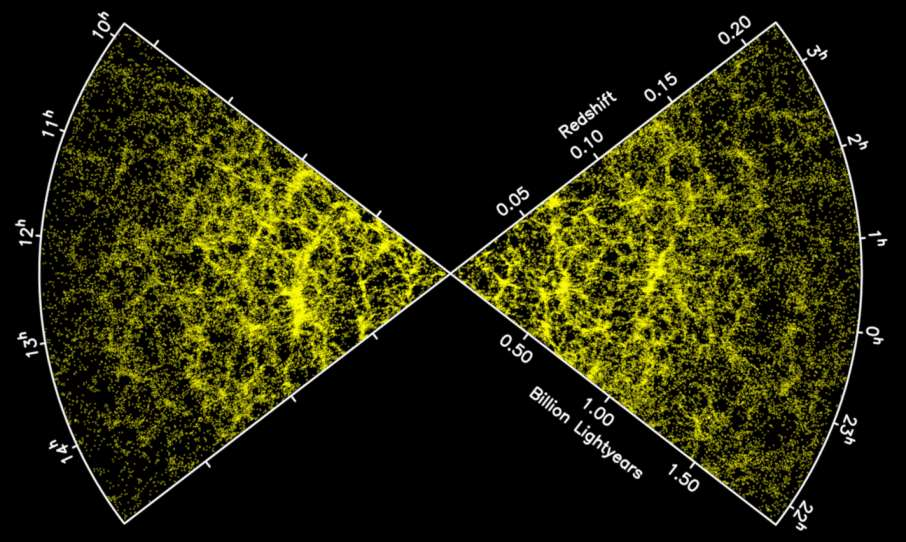
\includegraphics[width=4in]{chapter1/web_2df.jpg}}
\caption{The local ($z<0.2$) cosmic web as seen by the 2-degree-Field Redshift Survey. Each yellow dot is a galaxy with a spectroscopic redshift.}
\label{f:intro_web}
\end{figure}

The cosmological model introduced above predicts that structure grows hierarchically: small structures form first and then merge to give rise to larger structures. This continuous mass accretion and merging process has given rise to what we term the `Cosmic Web'. \Cref{f:intro_web} shows the local ($z<0.2$) cosmic web as seen by the 2-degree Field Galaxy Redshift Survey \citep{colless01}. At the intersections of this web lie galaxy clusters, the most massive gravitationally-bound structures formed so far in the Universe.

As the name suggests, galaxy clusters are objects in which galaxies abound---a massive cluster can host hundreds of bright galaxies \citep[e.g.,][]{abell58}. However, this simple description was rendered insufficient early on by \citeauthor{zwicky33} (\citeyear{zwicky33}, discussed above). We now know that galaxy clusters, with sizes of 1$-$2 Mpc and masses of up to a few times $10^{15}\,\Msun$, are mostly made of dark matter (roughly 80\% of their mass); only about 2\% of their mass is in stars, while the remaining 18\% is in a hot ionized gas with temperatures exceeding $10^7$ K that can be observed at X-ray wavelengths \citep[e.g.,][]{sarazin86}.


\section{Mass proxies and cosmological leverage}

Galaxy clusters can be used to quantify the ability of the Universe to aggregate matter and therefore serve as powerful cosmological probes. The number of clusters in the Universe at a given time---and their masses---depends on the matter density of the Universe, usually parametrized as $\Omega_{\rm m}\equiv\rho_{\rm m}/\rho_{\rm c}$ (where $\rho_{\rm c}$ is the `critical' density needed for the Universe to be flat), the size of density fluctuations left after the inflationary period, parametrized by $\sigma_8$, and the rate of expansion in the Universe, which can be quantified by the dark energy density, $\Omega_\Lambda\equiv\rho_\Lambda/\rho_{\rm c}$.

Exploiting clusters as cosmological probes requires knowledge of their masses, which is not an easy quantity to estimate. While gravitational lensing---the deflection of light due to the mass--induced curvature of space---provides a direct measurement of the surface mass density (which can be deprojected into a total mass under some assumptions), it has not been generally available for large samples of clusters.

Because of this, considerable effort has been devoted to characterize a variety of mass \emph{proxies}---observable quantities that, we hope, depend on mass in as simple a manner as possible, but also that are readily measurable with current capabilities. The most obvious of these is the number of galaxies, usually referred to as `richness', which has received considerable attention in recent years. Although initial attempts found that the richness was a very noisy mass proxy, recent studies have found that a properly-defined richness can be as good a proxy as any other \citep{rykoff12,andreon15}. Also common are X-ray--derived mass proxies, including the X-ray luminosity, the gas temperature and the gas mass. Of these, the gas mass shows the least scatter \citep{mahdavi13} but is the most difficult to obtain, and is currently only available for rather small samples.

A novel mass proxy, which has only been measurable in recent years thanks to new, sensitive high-resolution millimeter-wave surveys, is the Sunyaev-Zel'dovich \citep[SZ,][]{sunyaev72} effect.
% : the interaction of CMB photons with the hot electrons in galaxy clusters increases their energy, and creates `holes' in observations at frequencies around 150 GHz in the direction of galaxy clusters.
% The SZ effect is the inverse Compton scattering of CMB photons as they interact with the hot electrons in galaxy clusters. 
The SZ effect is produced by the interaction of CMB photons with the hot electrons in galaxy clusters; this interaction increases the energy of CMB photons and creates `holes' in observations at frequencies around 150 GHz in the direction of galaxy clusters. In a sense, therefore, observing the SZ effect is like seeing the shadow of a galaxy cluster. Because it is a CMB observable, the SZ surface brightness is independent of the redshift of the cluster producing it, and SZ surveys reveal the most massive clusters at all redshifts \citep{hasselfield13,bleem15}.\footnote{This is not true for the SZ survey carried out with the \planck\ satellite, which is mostly limited to $z<0.6$ \citep{planck15xxvii}. This is because high-redshift clusters have a small angular extent, so their SZ signal is diluted by the large beam of \planck\ (roughly $5'$).} In contrast, X-ray or optical observations reveal flux from the clusters themselves and are therefore generally limited to rather low redshift. In addition, the relation between SZ effect and mass has been predicted to have very little scatter \citep[at a level of 5--10\%; e.g.,][]{motl05,battaglia12}, although observations have shown that these predictions were rather optimistic \citep{benson13,sifon13}.

\begin{figure}
 \centerline{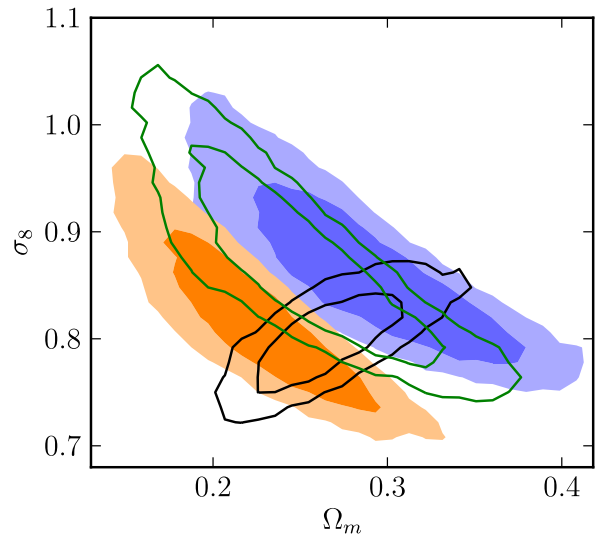
\includegraphics[height=2in]{chapter1/cosmo_SZ_ACT.png}
             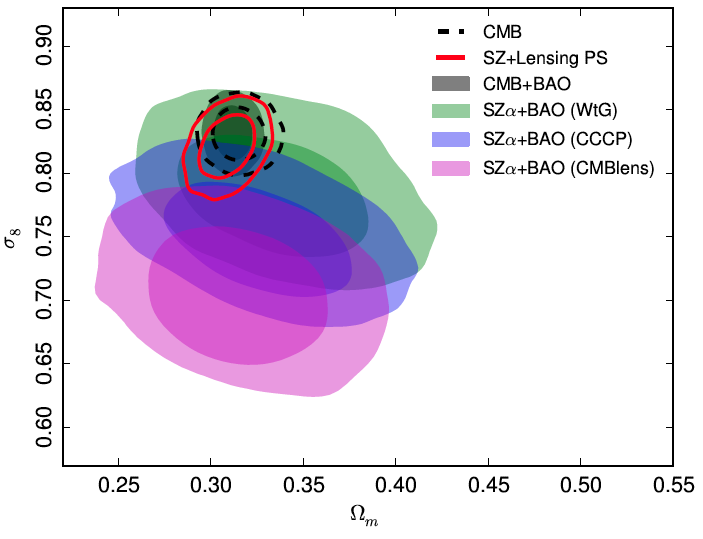
\includegraphics[height=2in]{chapter1/cosmo_SZ_Planck.png}}
\caption{Constraints on cosmological parameters $\Omega_{\rm m}$ and $\sigma_8$ from galaxy clusters detected by the Atacama Cosmology Telescope \citep[left, from][]{hasselfield13} and the \planck\ satellite \citep[right, from][]{planck15xxiv} through their SZ effect. Black contours in the left and right panel show constraints from primary CMB measurements by the WMAP and \planck\ satellites, respectively. The broader, coloured contours show different assumptions about the scaling between SZ effect and mass. Clearly, this dominates the uncertainty budget on cosmological parameters.}
\label{f:intro_szcosmo}
\end{figure}

Massive galaxy clusters at high redshift have a particularly strong leverage on cosmological parameters \citep{vikhlinin09_cosmo}, so SZ surveys are well-suited for cosmological parameter inference; the characterization of the SZ effect as a mass proxy is an active field of study. \Cref{f:intro_szcosmo} shows the constraints on cosmological parameters from galaxy clusters detected in the SZ survey by the Atacama Cosmology Telescope \citep[ACT,][]{hasselfield13} and the \planck\ satellite \citep{planck15xxiv}. Both analyses found that the main limitation to the constraining power is given by the unknown conversion from SZ effect to cluster mass (rather than statistical uncertainties), even though the ACT analysis is based on only 15 clusters. 


\section{Mass and light in cluster galaxies}

The galaxies we readily see in galaxy clusters tell us the story of a harsh, unforgiving environment: unlike the spiral galaxies (or `nebulae') known since time immemorial (but whose spiral nature was discovered by William Parsons, 3rd Earl of Rosse, in 1845, and whose physical properties have only been characterized over the course of the past century), galaxies in clusters are typically of elliptical shape and a distinct reddish colour \citep{dressler80,gladders00}. This difference arises because galaxies entering clusters suffer the fast removal of their cold ($\sim10$ K) gas (which can collapse to form stars); the galaxies are then left only with old stars, which on average look redder than the bluer young stars (hence the colour of spiral galaxies). 

This transformation is facilitated mainly by three distinct effects. \emph{Galaxy harassment} is the process by which a galaxy removes the gas from another galaxy due to a high-speed encounter or fly-by \citep{moore96}. \emph{Ram pressure stripping} is the removal of galactic gas by the gas in the intracluster medium, because the galaxy is traversing it at high speed \citep{gunn72,nulsen82}. Finally, \emph{strangulation} refers to the process by which the strong tidal forces produced by the gravitational potential of the cluster remove the cold gas from the galaxy \citep{larson80}. Whatever the exact relevance of each mechanism, these effects seem to remove the star formation fuel from galaxies on relatively short timescales of about 1 billion years or less \citep[e.g.][]{haines13,muzzin14}. Moreover, the evidence suggests that these effects are strong enough to suppress star formation even in low-mass galaxy groups \citep{haines15,balogh16}.


\subsection{Tidal effects on cluster galaxies}

Because galaxies do not follow radial orbits within clusters, they are subject to strong tidal torques from the cluster's gravitational potential. These torques have an effect on both the shapes and the masses of cluster galaxies.

Regarding the shapes, the tidal torques tend to align the galaxies such that their major axes point towards the centre of the host cluster. In numerical simulations of dark matter (where gravity is the only force present), this process is very efficient, and dark matter \emph{subhaloes} are tidally aligned with the host dark matter halo after the first pericentre passage, and remain aligned thereafter \citep[e.g.,][]{kuhlen07,pereira10}. However, simulations that incorporate gas and stars have shown that the case is not so clear-cut for galaxies. These simulations show that there is a degree of \emph{mis}alignment between the two components, such that the alignment of stellar light in galaxies is probably much weaker than that of the dark matter. Observational constraints on the strength of these cluster galaxy alignments, if any, can also have a strong impact on ongoing and upcoming cosmic shear surveys such as the Kilo-Degree Survey \citep[KiDS,][]{dejong15} or Euclid \citep{laureijs11}, as these \emph{intrinsic} alignments are anti-correlated with the apparent alignment of background sources produced by gravitational lensing \citep{hirata04}. If not accounted for, they could introduce significant biases on cosmological parameters inferred from cosmic shear measurements.

If the visible parts of galaxies undergo such dramatic changes when they become satellites, similar effects might apply to the dark component. Just like in isolated galaxies and galaxy clusters, dark matter is expected to be the dominant mass component in cluster galaxies; exactly how much so is not well known. In fact, the same tidal forces that might cause galaxies to align also act to transfer mass from the satellite galaxy to the host cluster. Statistical measurements of this \emph{tidal stripping} effect are particularly challenging: in addition to the difficulty of measuring the masses of galaxies in general, one must be able to identify galaxies belonging to clusters in the first place.

Measuring the total masses of cluster galaxies has implications not only for models of galaxy formation and evolution, but also for cosmology. Specifically, the energy of the postulated dark matter particle defines the amount of mass that is contained in substructures within the large scale structure (i.e., galaxies in clusters, or satellite galaxies around massive galaxies). A universe where dark matter is ``warm'' produces less substructure than one where dark matter is ``cold'' \citep[e.g.,][]{libeskind13}. Therefore the fraction of mass in cluster galaxies (relative to the total mass of a galaxy cluster) depends on the energy of the dark matter particle. %Large-scale structure measurements suggest that our Universe contains cold dark matter \citep[e.g.,][]{blumenthal84}, and accurate measurements of cluster galaxy masses would provide a complementary test of this.
The cold dark matter model provides a good description of large-scale structure observations and is the most widely-accepted scenario \citep[e.g.,][]{blumenthal84,frenk12}; accurate measurements of cluster galaxy masses would provide a complementary test of it.


\section{This thesis}

In this thesis we use a variety of observations and techniques to study the connection between the mass and light contents of galaxy clusters from different perspectives. The implications of different aspects of this connection have been briefly outlined above and are discussed in more detail in each chapter.

In \citechapter{2} we characterize \plck, a galaxy cluster recently discovered by the \planck\ satellite through its SZ effect. We present the first optical images of this cluster, measure its redshift ($z=0.52$) and identify multiple images of a lensed background galaxy, which allows us to perform a strong lensing analysis. We also show that \plck\ hosts diffuse radio emission---the tell-tale sign of cluster mergers and, to this day, an extremely rare sight at $z>0.4$.

In \citechapter{3} we use extensive spectroscopic observations of galaxy clusters detected through the Sunyaev-Zel'dovich effect to measure the velocity dispersions of their member galaxies. Taking previous results from hydrodynamical simulations, we convert these velocity dispersions into cluster masses and compare them to the strength of the SZ effect, with the aim of characterizing the latter to allow its use for cosmological parameter inference. We pay particular attention to sources of uncertainty and scatter in the determination of the velocity dispersions, and conclude that the dominant uncertainty comes from the identification of member galaxies, which poses an irreducible uncertainty on velocity dispersions as mass proxies.

In the second half of this thesis we turn our attention to the galaxies residing in clusters. In particular, in \citechapter{4} we investigate the alignment of the shapes of cluster galaxies. We base our study on a sample of 90 clusters with deep, wide-field observations devised for accurate weak lensing measurements. We first perform a thorough literature search for spectroscopic redshifts with which to select galaxies physically belonging to these clusters, resulting in a sample of more than 14,000 cluster galaxies. We then measure the orientations of cluster galaxies to see if there are any signs of alignment of galaxies within clusters.

In \citechapter{5} we exploit the overlap between the spectroscopic Galaxy And Mass Assembly survey (GAMA) and the deep photometric Kilo-Degree Survey to measure the masses of satellite galaxies in galaxy groups using weak gravitational lensing, with the aim of constraining the segregation of group galaxies by mass. The spectroscopic nature of the galaxy group catalogue ensures we can do this essentially free of contamination from both non-group galaxies and central galaxies.

Finally, in \citechapter{6} we extend the lensing measurements of \citechapter{5} to more massive galaxy clusters using the dataset produced for \citechapter{4}. Using weak lensing measurements of the masses of cluster galaxies, we constrain the stellar-to-subhalo mass relation and study the mass segregation of cluster galaxies.


% \section{Concluding remarks}
% 
% Observation